
    \subsection*{Параметры: $T=3$, $\Delta t=0.05$, $V=20$, $\Delta \nu=0.01$}

    \begin{figure}[H]
        \centering
        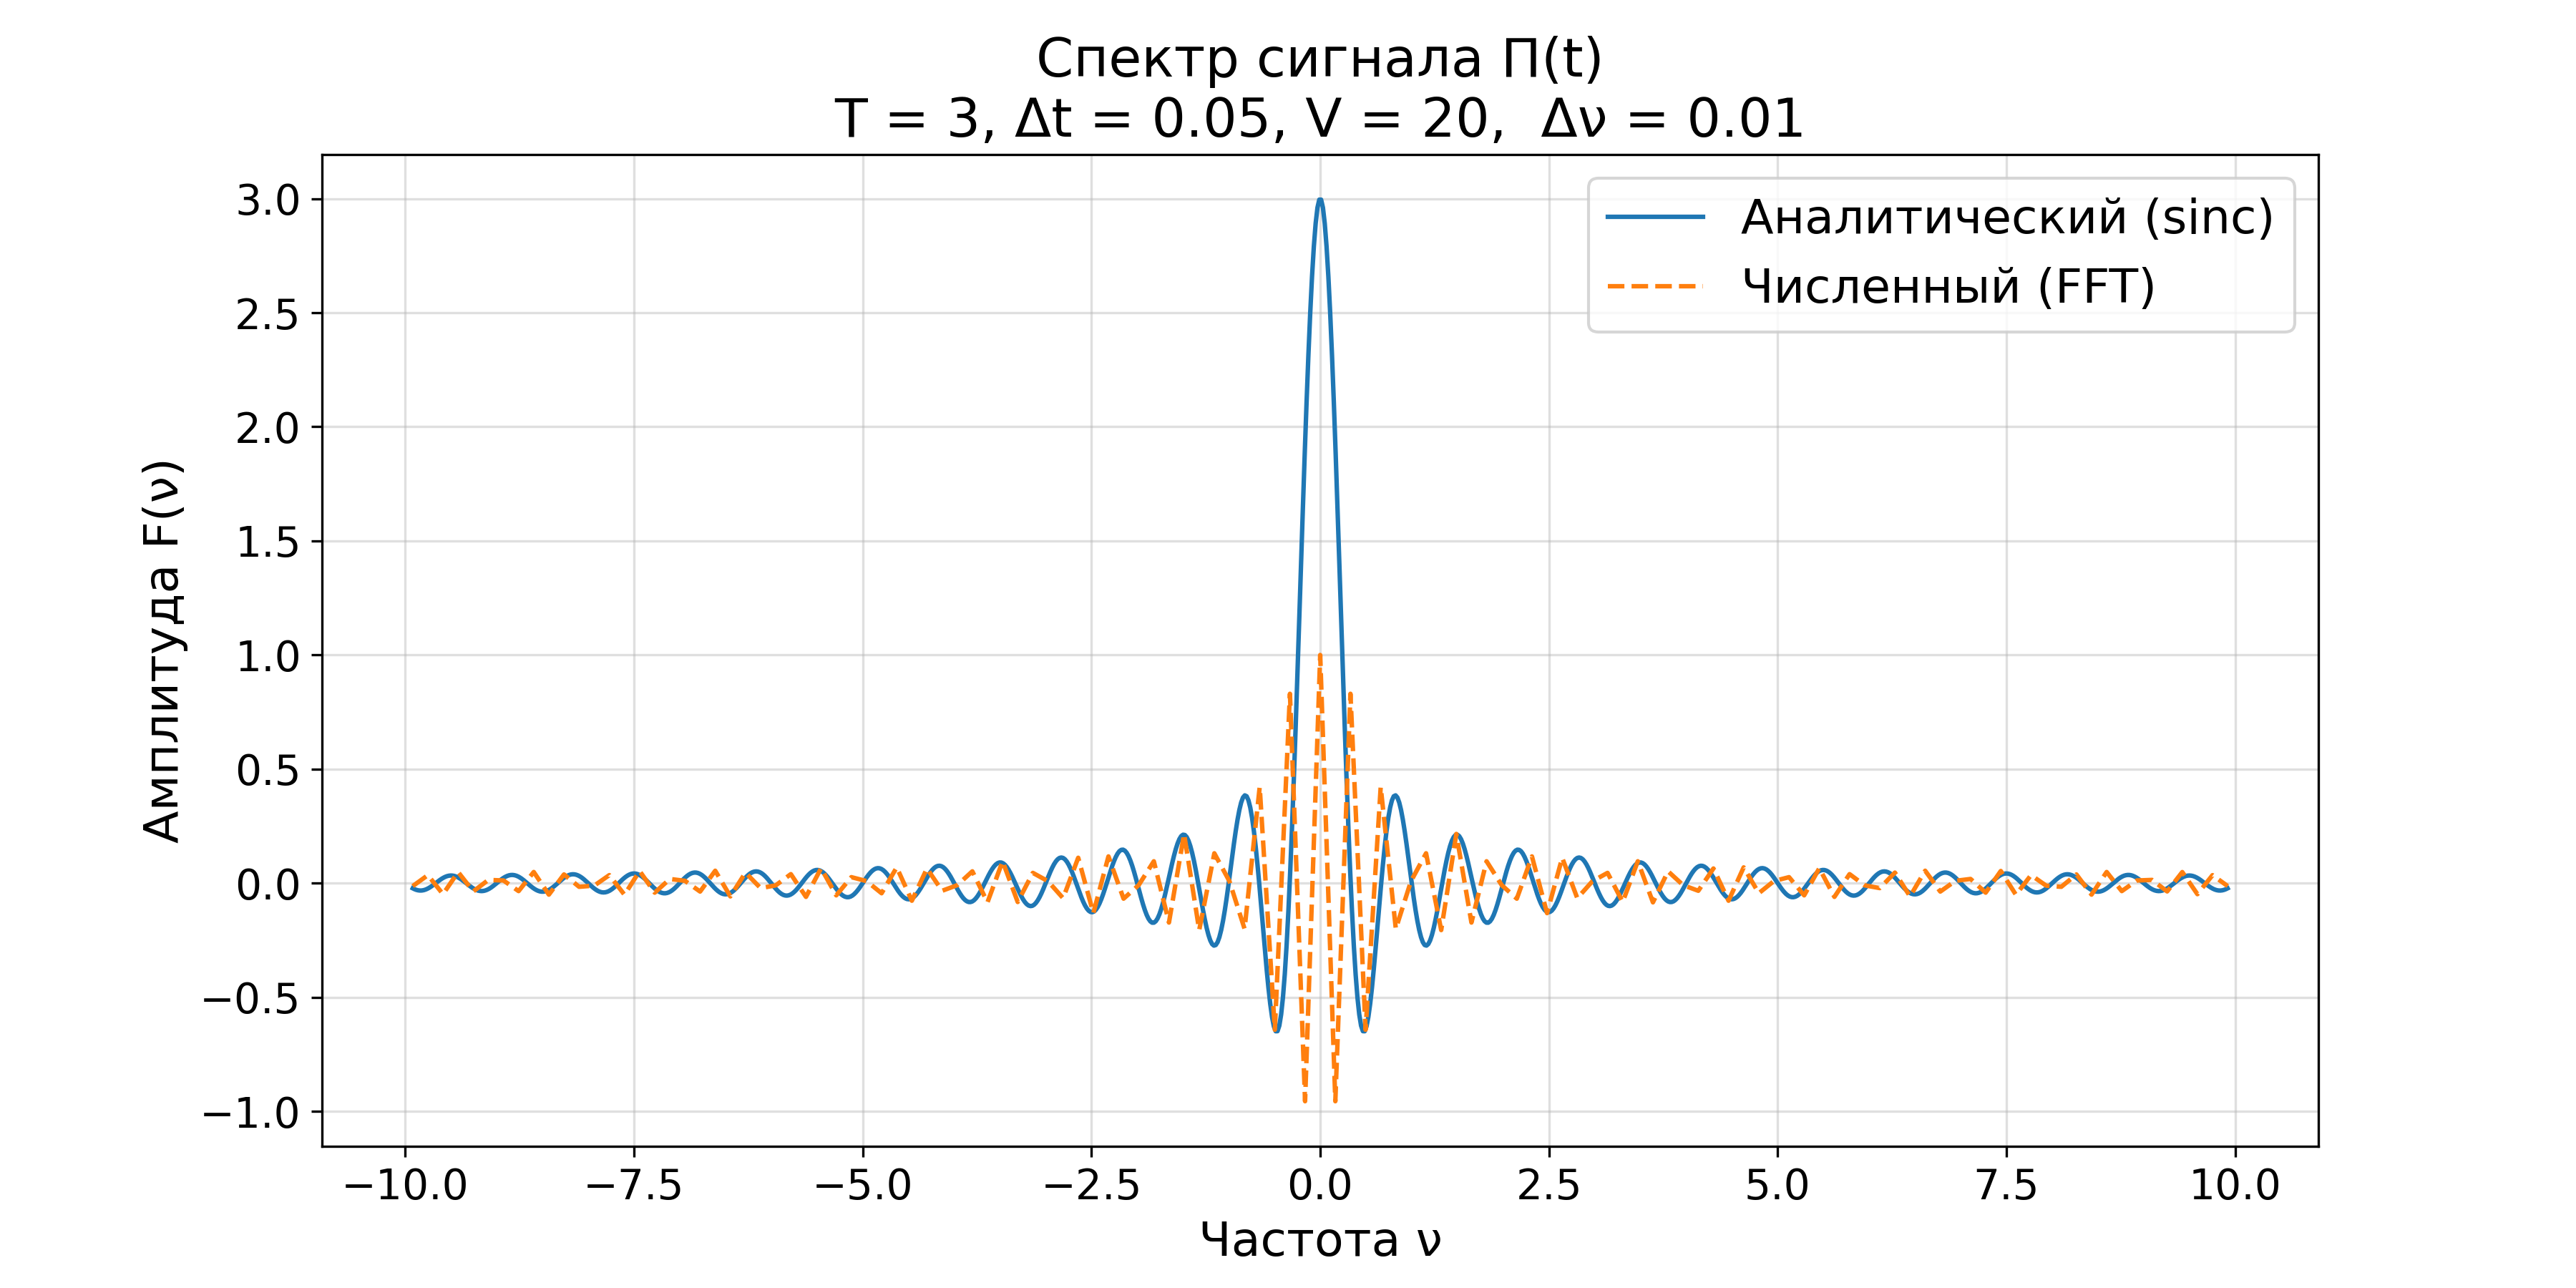
\includegraphics[width=0.8\textwidth]{task1/figs_1_5/1_5_set_8_spectrum.png}
        \caption{Спектр сигнала $\Pi(t)$ (численный FFT и аналитический sinc)}
    \end{figure}

    \begin{figure}[H]
        \centering
        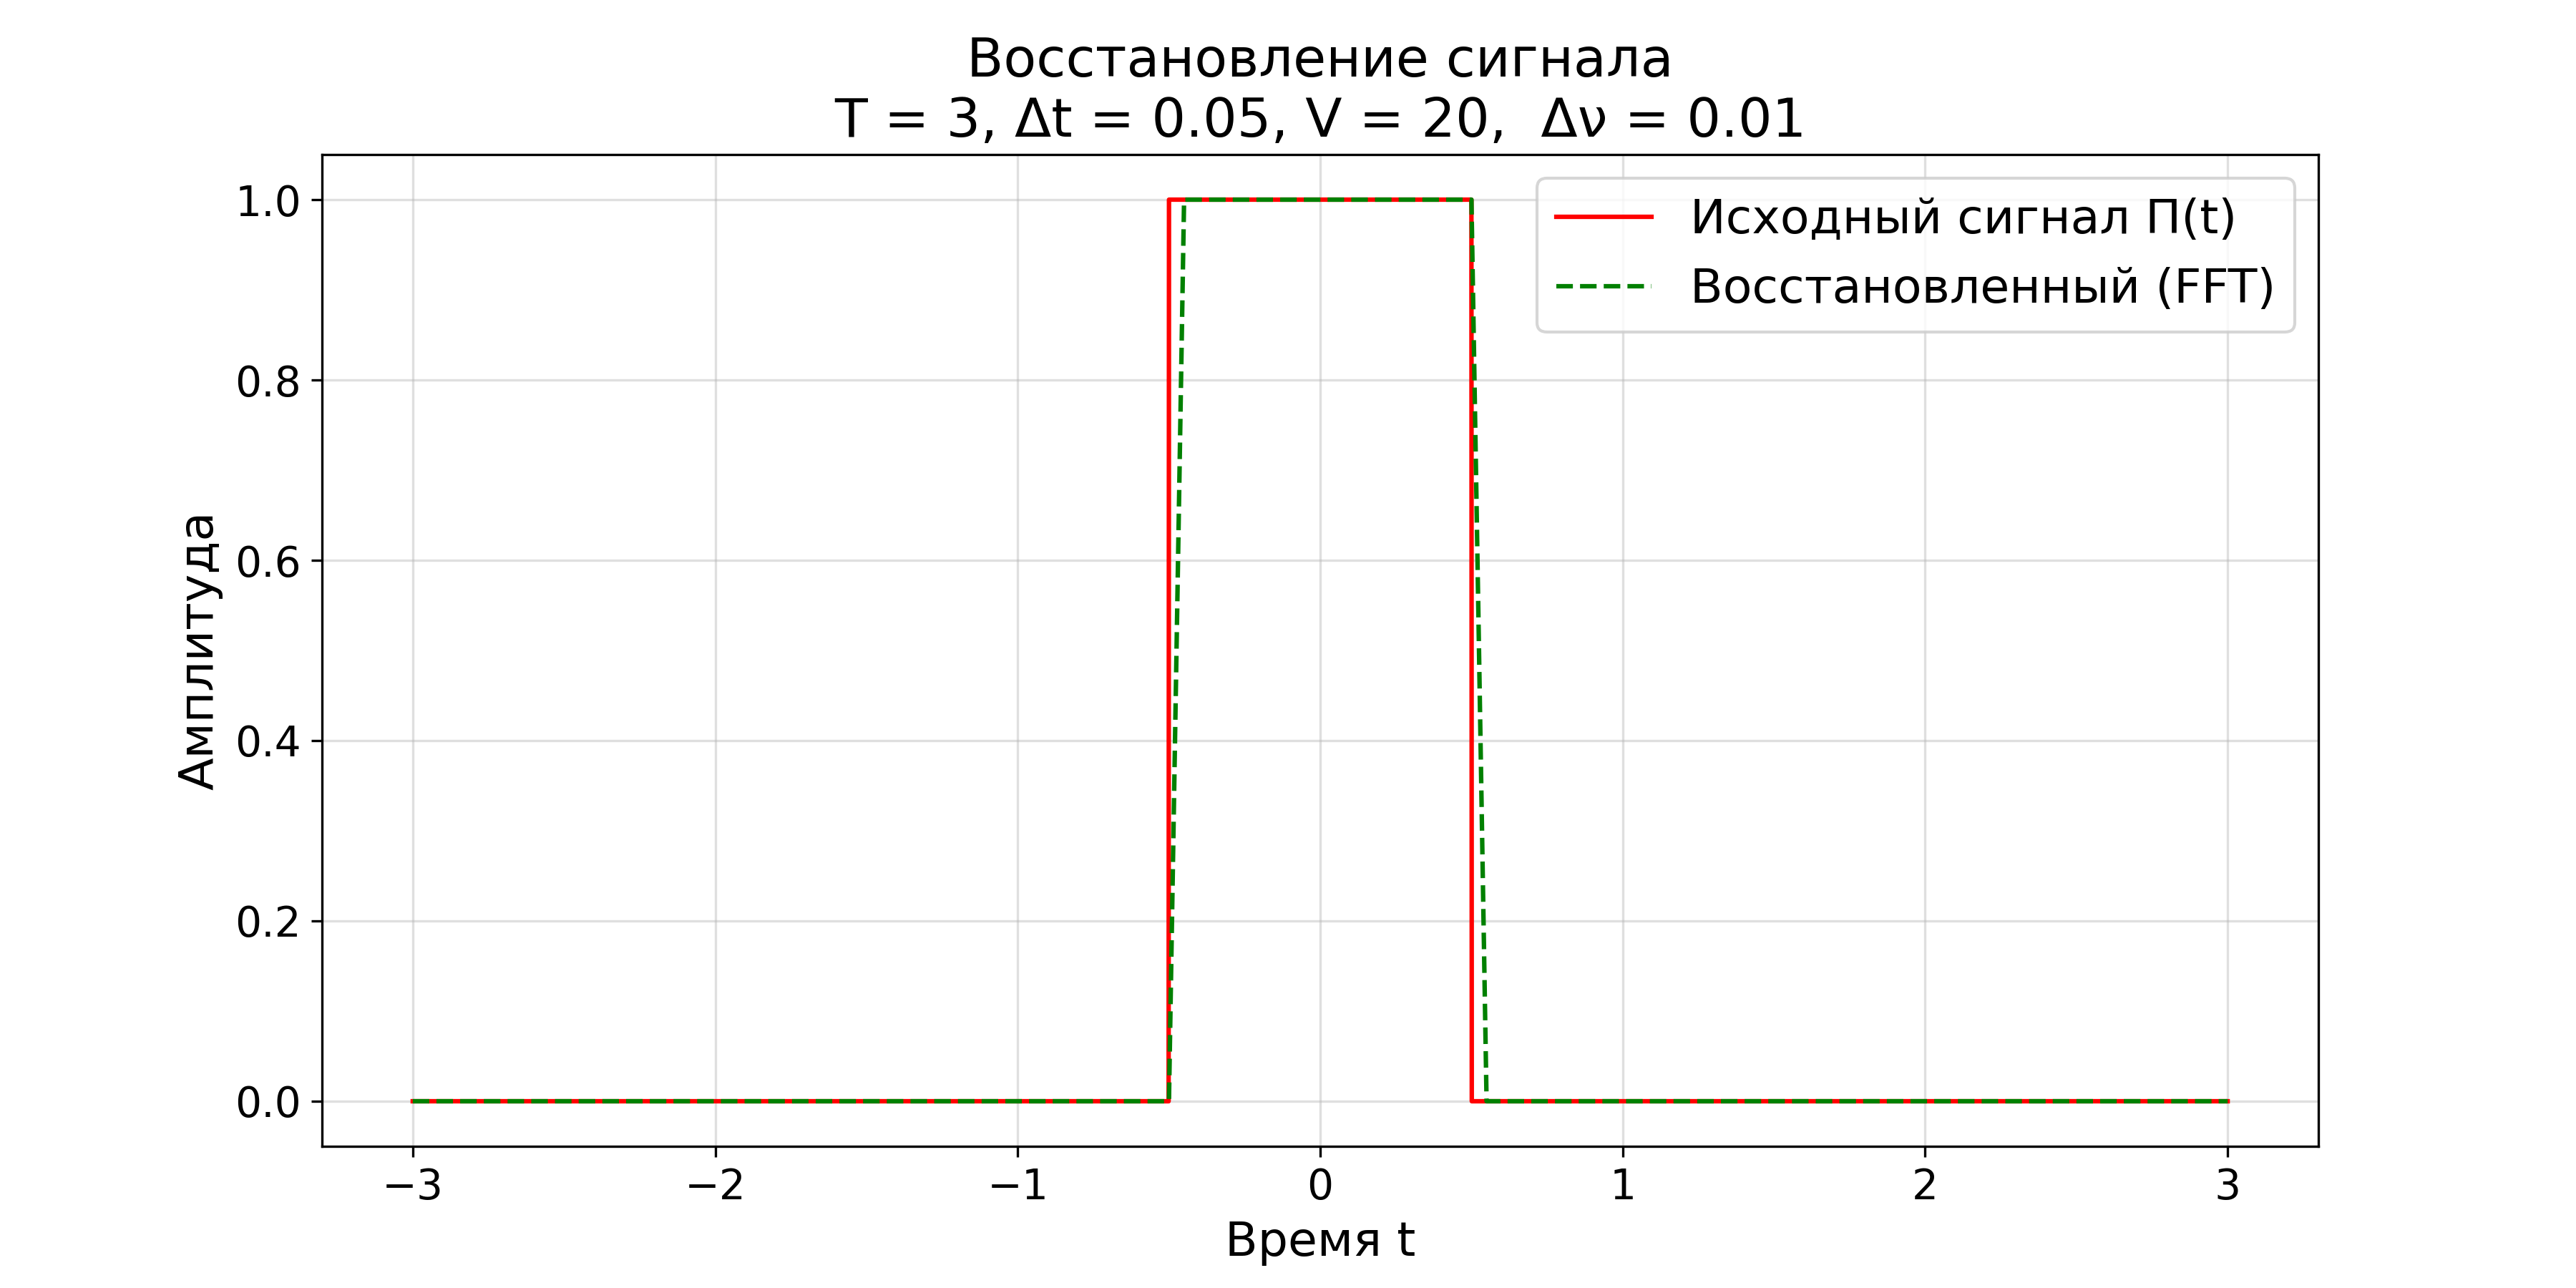
\includegraphics[width=0.8\textwidth]{task1/figs_1_5/1_5_set_8_reconstruction.png}
        \caption{Восстановление сигнала $\Pi(t)$ методом FFT}
    \end{figure}
    